% Experiment 3: six square marginals, colour fixed by G_intersection.
% ColorBrewer PuOr: orange \#f1a340 and purple \#998ec3.
\begin{figure}[H]
\centering
\rule{\textwidth}{0.4pt}\\[3pt]
\begin{tabular*}{\textwidth}{@{\extracolsep{\fill}}ccc@{}}
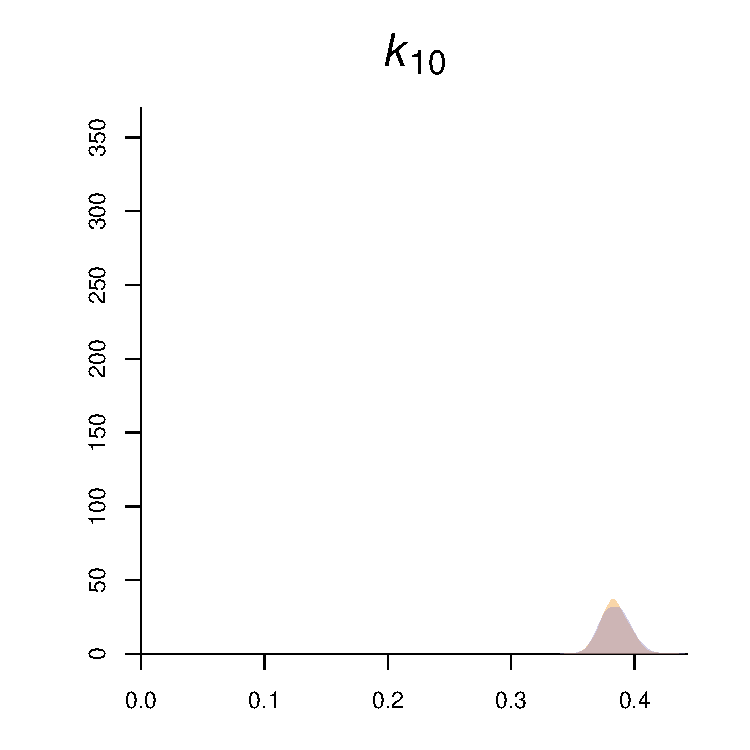
\includegraphics[width=4cm,height=4cm]{fig_experiment3_k10.pdf} &
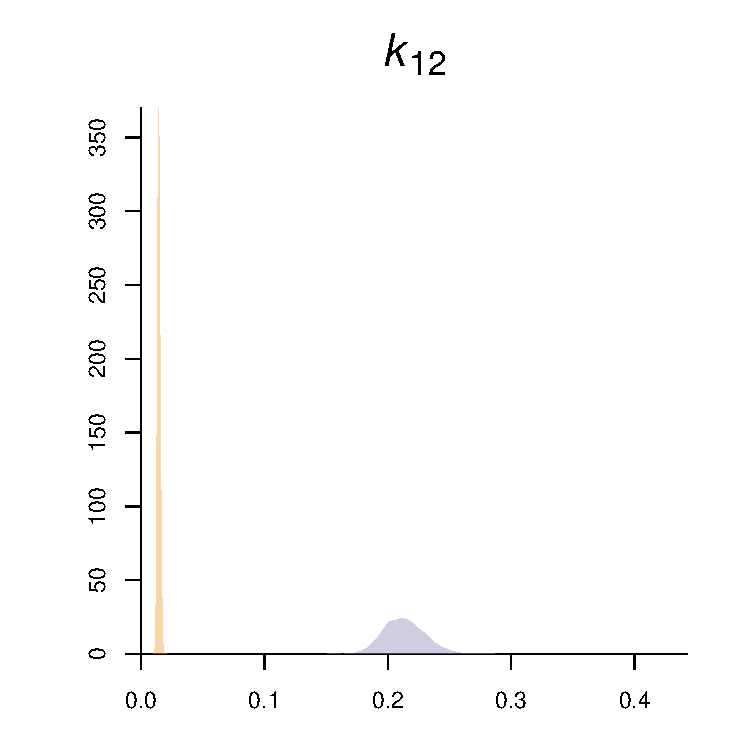
\includegraphics[width=4cm,height=4cm]{fig_experiment3_k12.pdf} &
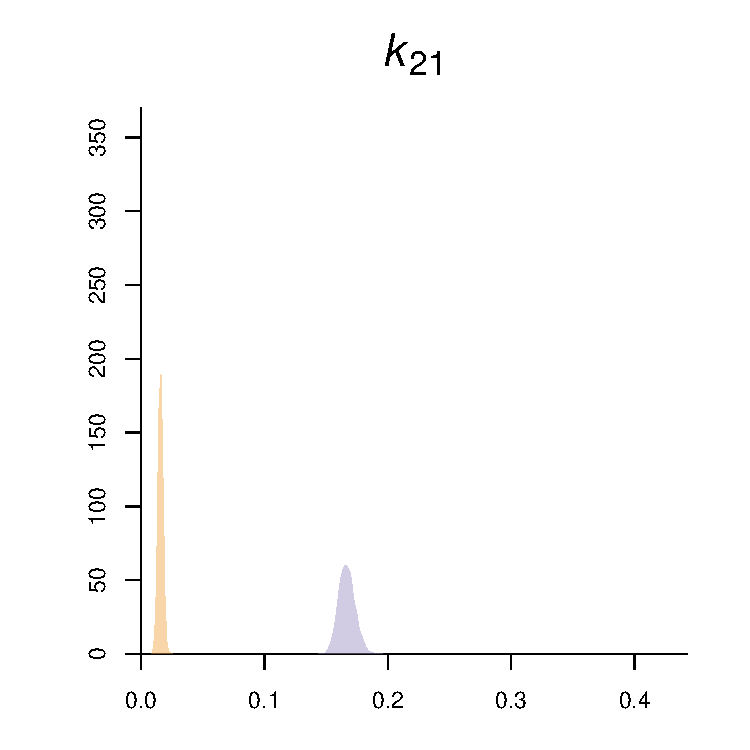
\includegraphics[width=4cm,height=4cm]{fig_experiment3_k21.pdf} \\[4pt]
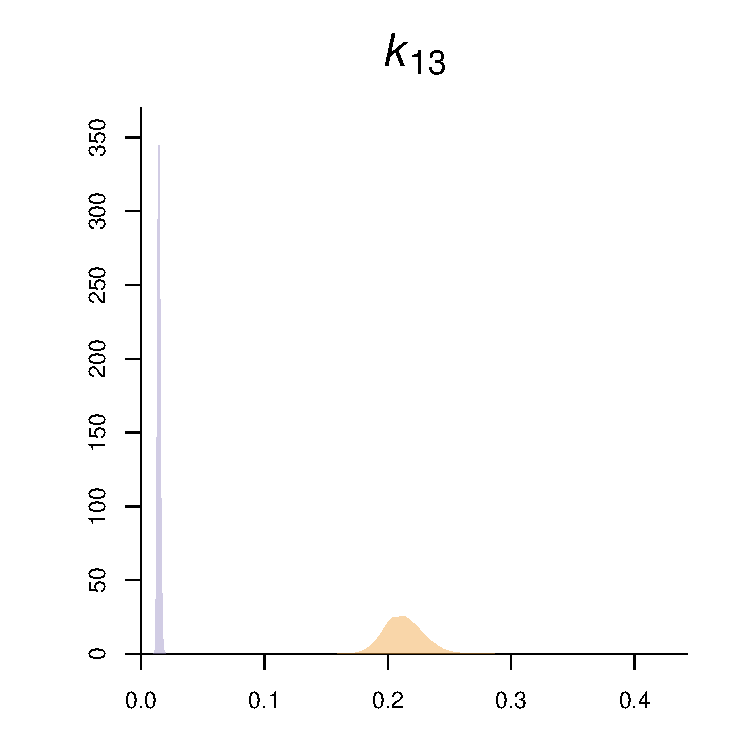
\includegraphics[width=4cm,height=4cm]{fig_experiment3_k13.pdf} &
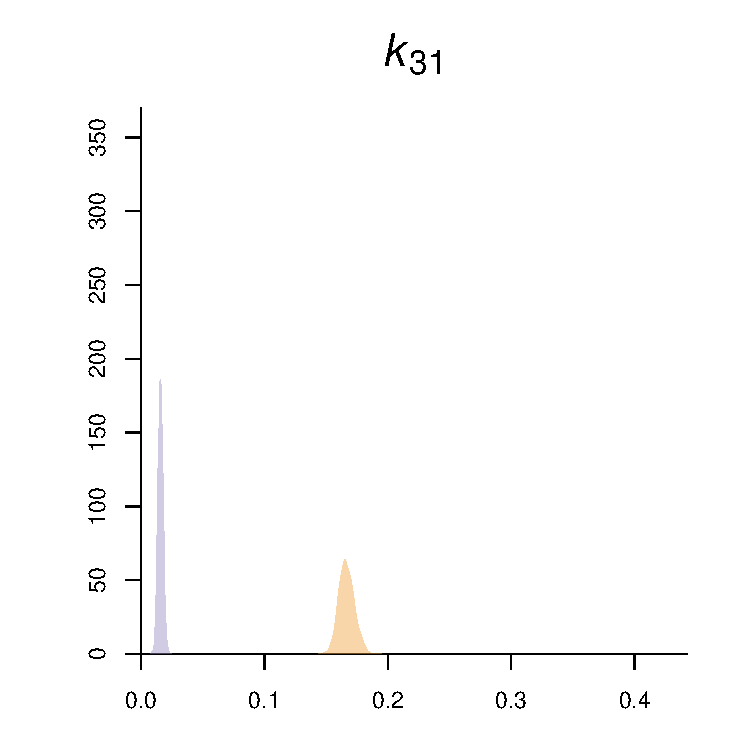
\includegraphics[width=4cm,height=4cm]{fig_experiment3_k31.pdf} &
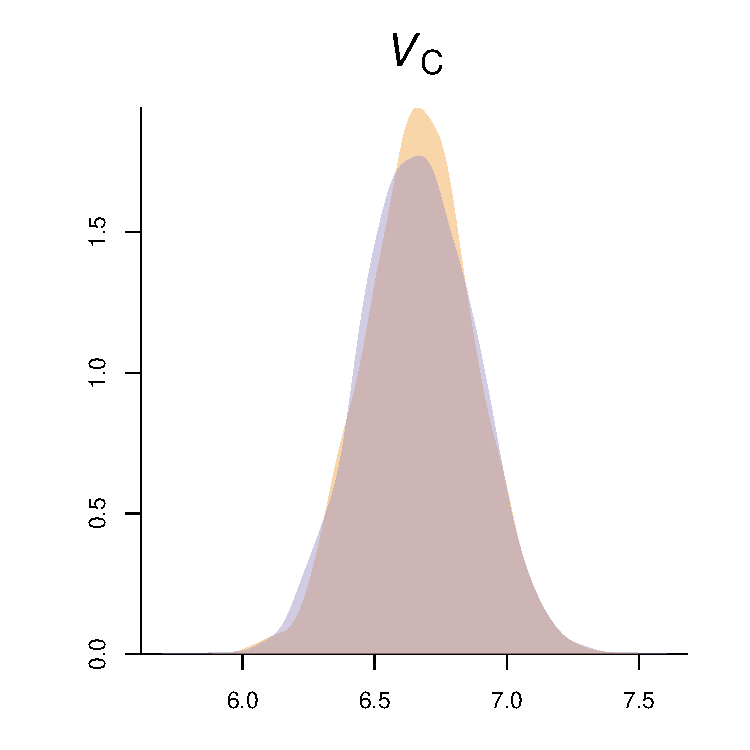
\includegraphics[width=4cm,height=4cm]{fig_experiment3_VC.pdf}
\end{tabular*}\\[3pt]
\rule{\textwidth}{0.4pt}
\caption{%
\textbf{Marginal posteriors of the rate parameters in the
three-compartment pharmacokinetic model.}
Colour marks the two connected components of $G_\cap$:
orange for one chain group and purple for the other.
The same chain-to-colour map is used in every panel.
}
\label{fig:experiment3-marginals}
\end{figure}
